\documentclass[a4paper,11pt,twoside]{article}
%\documentclass[a4paper,11pt,twoside,se]{article}

\usepackage{UmUStudentReport}
\usepackage{verbatim}   % Multi-line comments using \begin{comment}
\usepackage{courier}    % Nicer fonts are used. (not necessary)
\usepackage{pslatex}    % Also nicer fonts. (not necessary)
\usepackage[pdftex]{graphicx}   % allows including pdf figures
\usepackage{listings}
\usepackage{pgf-umlcd}
\usepackage{amsmath}
\usepackage{amsfonts}
\usepackage{amssymb}
%\usepackage{lmodern}   % Optional fonts. (not necessary)
%\usepackage{tabularx}
%\usepackage{microtype} % Provides some typographic improvements over default settings
%\usepackage{placeins}  % For aligning images with \FloatBarrier
%\usepackage{booktabs}  % For nice-looking tables
%\usepackage{titlesec}  % More granular control of sections.

% DOCUMENT INFO
% =============
\department{Department of Computing Science}
\coursename{Language and Computation 7.5 p}
\coursecode{5DV162}
\title{Assignment 1}
\author{Lorenz Gerber ({\tt{dv15lgr@cs.umu.se}}, {\tt{lozger03@student.umu.se})}}
\date{2016-09-20}
%\revisiondate{2016-01-18}
\instructor{Henrik Björklund}


% DOCUMENT SETTINGS
% =================
\bibliographystyle{plain}
%\bibliographystyle{ieee}
\pagestyle{fancy}
\raggedbottom
\setcounter{secnumdepth}{2}
\setcounter{tocdepth}{2}
%\graphicspath{{images/}}   %Path for images

\usepackage{float}
\floatstyle{ruled}
\newfloat{listing}{thp}{lop}
\floatname{listing}{Listing}



% DEFINES
% =======
%\newcommand{\mycommand}{<latex code>}

% DOCUMENT
% ========
\begin{document}
\lstset{language=C}
\maketitle
\thispagestyle{empty}
\newpage
%\tableofcontents
%\thispagestyle{empty}
%\newpage

\clearpage
\pagenumbering{arabic}

\section*{Problem 1} 
Assume that $L$ is a regular language. Strings $w$ of language $L$ are constructed according to the specification where zero, one or several $a$'s and zero, one or several $b$s are mixed freely as long as there are more $b$'s than $a$'s in it. Let's have a look at such a generic string and how it can be split into three parts $xyz$ such that $xy$ is shorter than $m$, $x$ is $1$ or larger and all $xy^{i}z$ are part of $L$ for all $i \in \mathbb{N}$. Independent of how $m$ is chosen, if $y$ contains more $a$'s than $b$'s, which according to the language definition is possible,  the resulting strings for $xy^{i}z$ $i \in \mathbb{N}$  are for large enough $i$ no longer part of $L$. Hence, proven by contradiction, $L$ can not be a regular language. 

\section*{Problem 2}
Assume that $L$ is a regular language. Strings $w$ of language $L$ are constructed according to the specification as $a^n$ with $n$ being a prime number equal or larger than $2$. For every prime $n$, there has to be a number $m$ which is smaller than $n$, and that multiplied with any natural number plus the difference $n - m$ will be a prime. Such a number does not exist. Hence, L can not be a regular language. 

The above is my initial solution. After some research on the net I
happend to find an exact formal solution to the problem \cite{pumpprime}. It took some
time until I understood it but now I do and therefore I reproduce it
here, though,  admitting that I probably could not have come up with it by
myself. 
 
\begin{enumerate}
\item Assume $L$ is regular, hence there has to be an $m$
\item choose a word $w=a^{n}$ where $n$ is a prime and $|xyz| = n >
  m+1$ (comment: The `$m+1$' part seems to be the critical assumption which I hardly could have come up with).
\item as $|xy| \leqslant m$ it follows that $|z| > 1$
\item as $|z| > 1$ it follows that $|xy| > 1$. Now choose $i =
  |xy|$. Then $|xy^{i}z| = |xy|+|y||xz|=(1+|y|)$. As $(1+|y|)$  and
  $|xy|$ are both greater than 1, the product must be a composite
  number. Hence$|xy^{i}z|$ is a composite number and not a prime.
\end{enumerate}


\section*{Problem 3}
Conversion of context free grammar into Chomsky normal form:

First Rule 1 is applied;

\begin{flalign*}
  &S \rightarrow aAB\\
  &A \rightarrow aAa\\
  &A \rightarrow bb\\
  &B \rightarrow a \\
\end{flalign*}

\begin{flalign*}
  &S_0 \rightarrow aAB\\
  &S \rightarrow aAB\\
  &A \rightarrow aAa | bb\\
  &B \rightarrow a\\
\end{flalign*}

No application for the epsilon and unit rule. The last shown steps are according rule four:

\begin{flalign*}
  &S_0 \rightarrow BAB\\
  &S \rightarrow BAB\\
  &A \rightarrow BAB | bb\\
  &B \rightarrow a\\
\end{flalign*}

\begin{flalign*}
  &S_0 \rightarrow BU\\
  &S \rightarrow BU\\
  &A \rightarrow BU | bb\\
  &U \rightarrow AB\\
\end{flalign*}

\begin{flalign*}
  &S_0 \rightarrow BU\\
  &S \rightarrow BU\\
  &A \rightarrow BU | bb\\
  &U \rightarrow AB\\
  &V \rightarrow b\\
\end{flalign*}

\section*{Problem 4}
Proving that the resulting Language $Ls$ from shuffeling the regular languages $L1$ and $L2$ is also regular was attempted here by construction.

The idea is to construct a NFA from NFA/DFA's that accept $L1$ and $L2$. Let's assume The wordlength of $L1$ and $L2$ is $|w1|$ and $|w2|$, hence the NFA/DFA to accept $L1$ or $L2$ will have $u_{1} \ldots u_{|w1|}$ respectively $v_{1} \ldots v_{|w2|}$ states. Now, for example state u1 is split into $|w1|$ substates to `remember' how many states of NFA 2 already have been passed. The same is done for all states of the NFA 1 and 2. Hence the new NFA will in this case have 18 + 2 states (18 + start and accepted end state). All inbound transitions are the same as in the initial NFA's. Hence it has been proven by construction of a new NFA that the shuffle of $L1$ and $L2$ is also a regular language.

The solution is shown in figure 1 produced with graphviz \cite{graphviz}. Figure 2 shows a hand draft of the same figure, but with a more clear grouping.

\begin{figure}
  \centering
  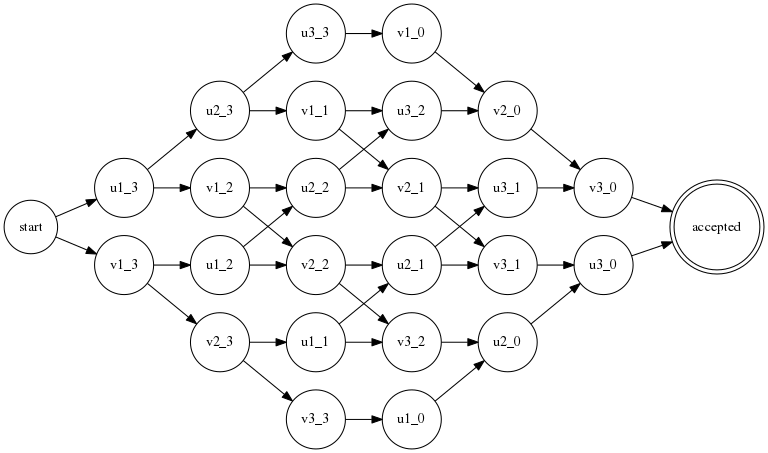
\includegraphics[width=\textwidth]{graph}
  \caption{\textit{Non-Deterministic Finite Automaton of shuffle between L1 and L2, generated with graphviz.}}
  \label{fig:graph}
\end{figure}

\begin{figure}
  \centering
  \includegraphics[width=\textwidth]{draft}
  \caption{\textit{Non-Deterministic Finite Automaton of shuffle between L1 and L2, hand draft.}}
  \label{fig:graph}
\end{figure}

\addcontentsline{toc}{section}{\refname}
\bibliography{references}

\end{document}
 
